% 本源与 SVG 使用相同数据与布局；尚未在本轮编译或视觉验收。
% 在配置完整的 TeX Live 环境中，进入本文件目录执行：
% xelatex -halt-on-error -interaction=nonstopmode bpe-learning-vs-encoding.tex
\documentclass[tikz,border=4pt]{standalone}
\usepackage{fontspec}
\setmainfont{TeX Gyre Heros}
\setsansfont{TeX Gyre Heros}
\setmonofont{Latin Modern Mono}
\usepackage{xcolor}
\usetikzlibrary{arrows.meta}
\definecolor{colorf7fafc}{HTML}{f7fafc}
\definecolor{color192b42}{HTML}{192b42}
\definecolor{color52677c}{HTML}{52677c}
\definecolor{colorffffff}{HTML}{ffffff}
\definecolor{colord7e1ea}{HTML}{d7e1ea}
\definecolor{colordcf2eb}{HTML}{dcf2eb}
\definecolor{color9ecdbd}{HTML}{9ecdbd}
\definecolor{coloreff3f7}{HTML}{eff3f7}
\definecolor{color25836d}{HTML}{25836d}
\definecolor{colorb9c8d7}{HTML}{b9c8d7}
\definecolor{colore0ebfa}{HTML}{e0ebfa}
\definecolor{colorfff3dc}{HTML}{fff3dc}
\definecolor{color9ab8de}{HTML}{9ab8de}
\definecolor{color4c78aa}{HTML}{4c78aa}
\definecolor{color8a641f}{HTML}{8a641f}
\begin{document}
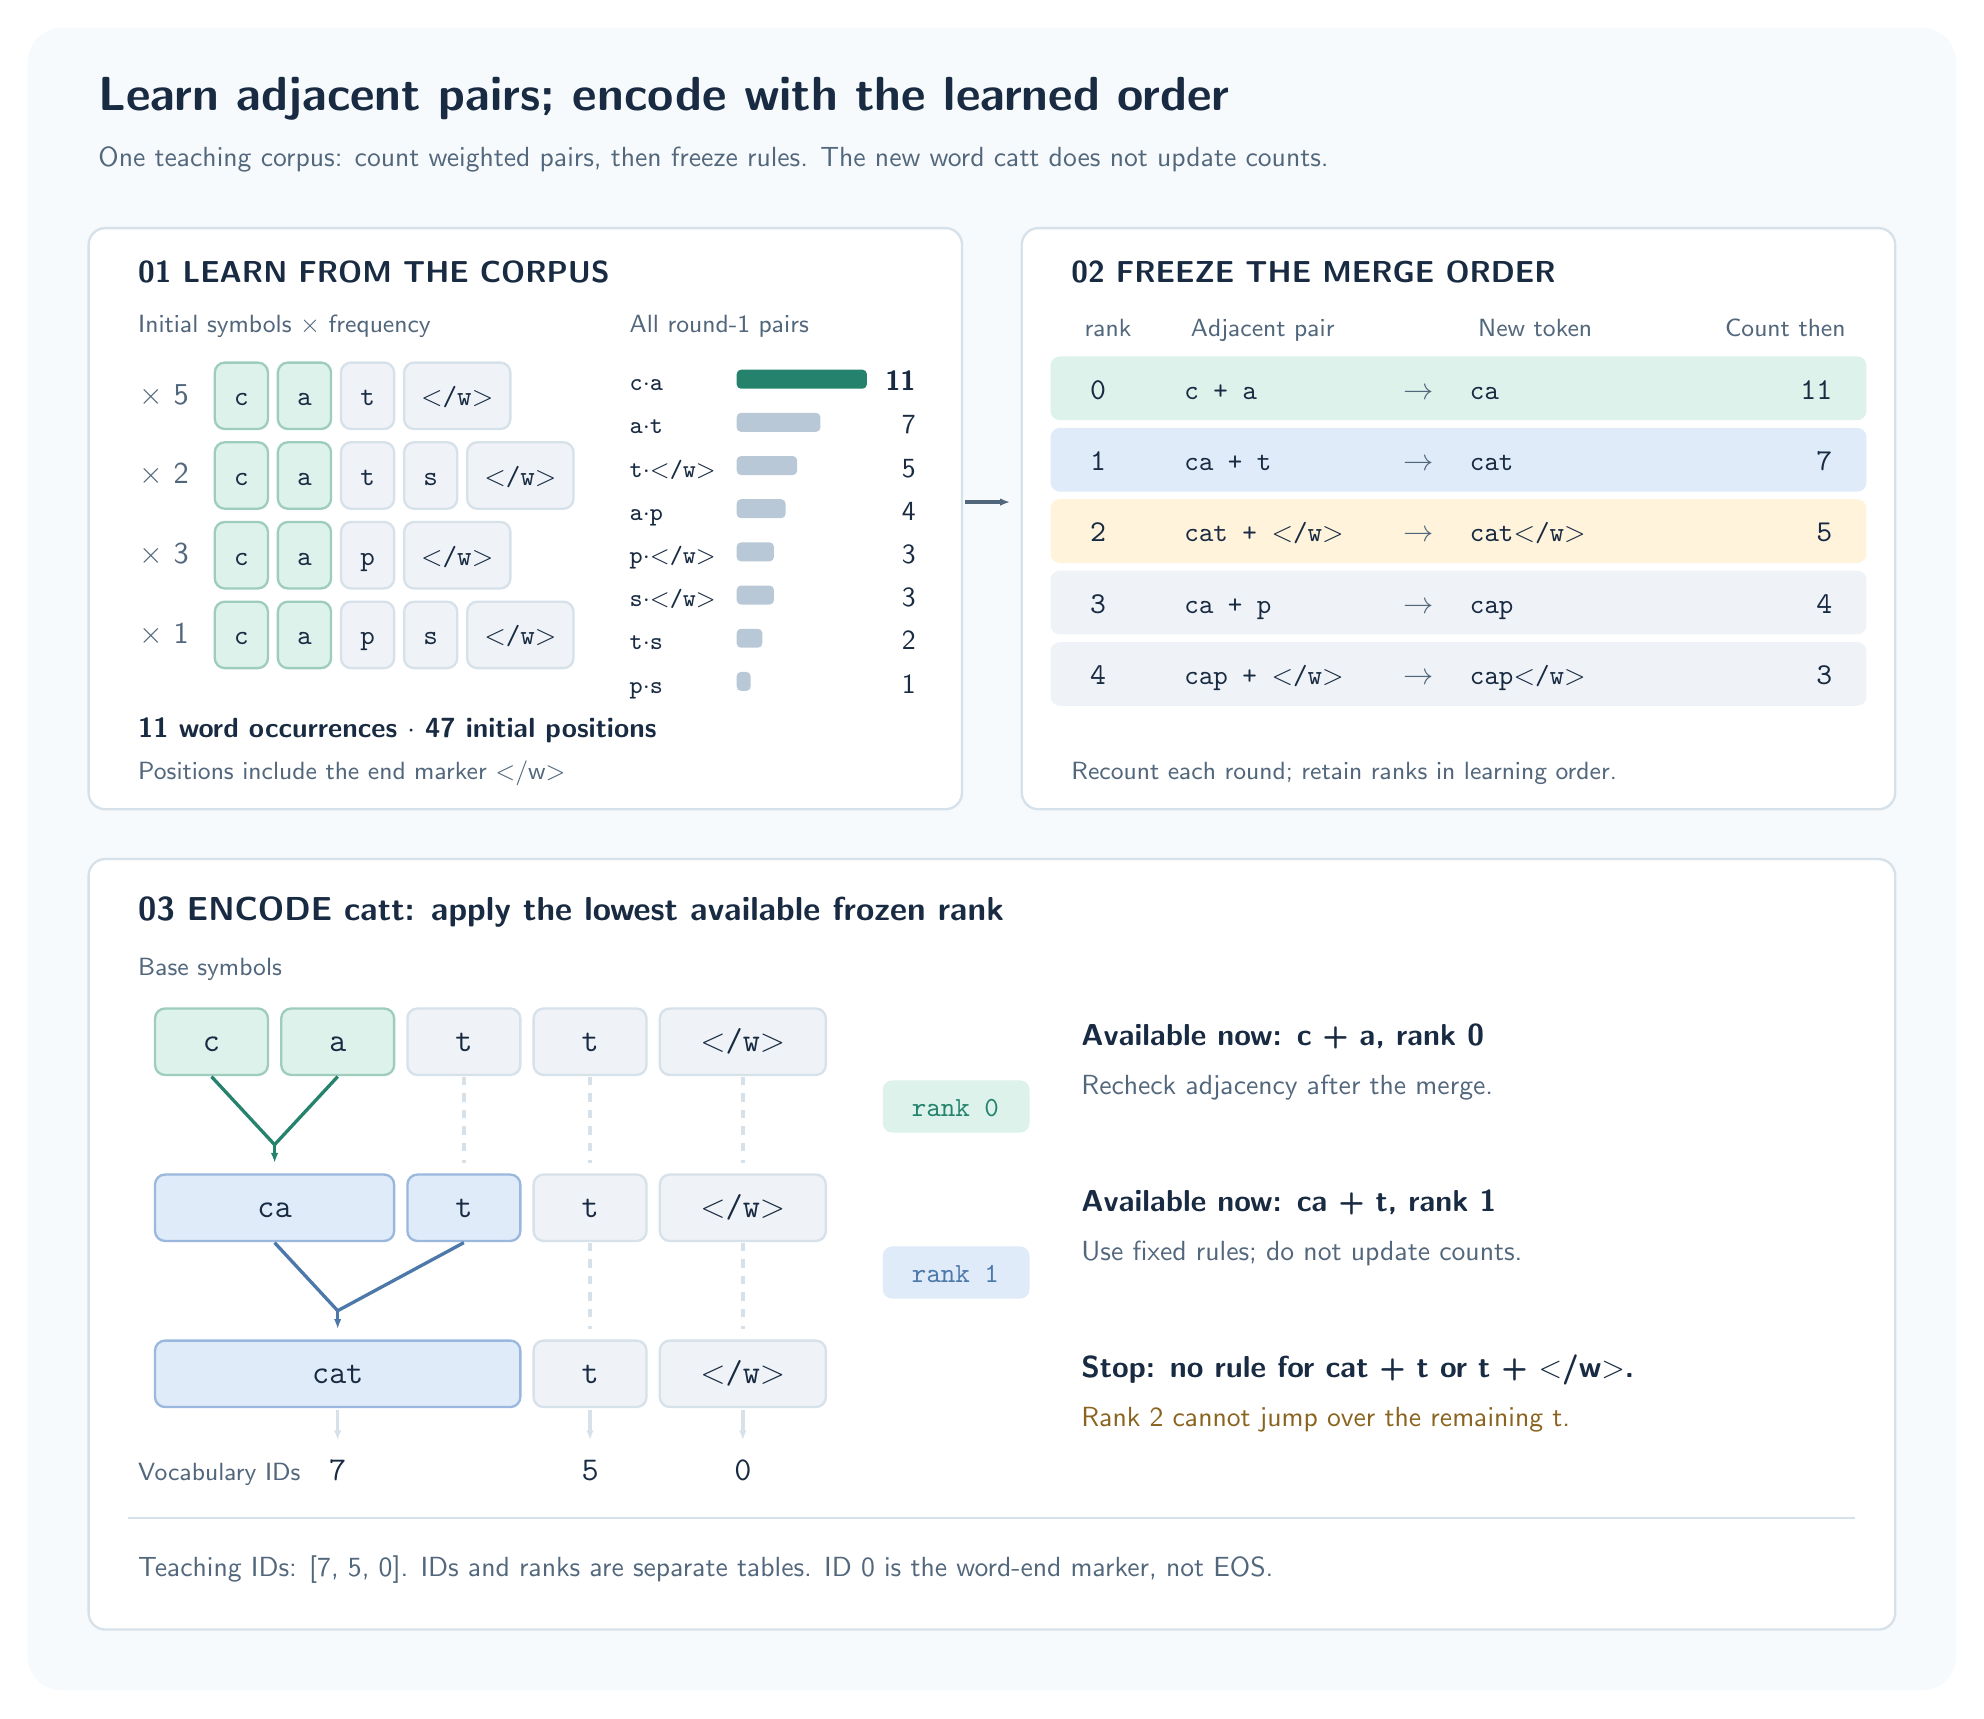
\begin{tikzpicture}[x=.6pt,y=-.6pt]
\path[fill=colorf7fafc,draw=colorf7fafc,line width=.84pt,rounded corners=12pt] (0,0) rectangle (1160,1000);
\node[anchor=base west,text=color192b42,font=\sffamily\fontsize{17.4}{22.62}\selectfont\bfseries] at (36,49) {Learn adjacent pairs; encode with the learned order};
\node[anchor=base west,text=color52677c,font=\sffamily\fontsize{10.2}{13.26}\selectfont] at (36,83) {One teaching corpus: count weighted pairs, then freeze rules. The new word catt does not update counts.};
\path[fill=colorffffff,draw=colord7e1ea,line width=.84pt,rounded corners=6pt] (36,120) rectangle (562,470);
\path[fill=colorffffff,draw=colord7e1ea,line width=.84pt,rounded corners=6pt] (598,120) rectangle (1124,470);
\node[anchor=base west,text=color192b42,font=\sffamily\fontsize{11.4}{14.82}\selectfont\bfseries] at (60,153) {01 LEARN FROM THE CORPUS};
\node[anchor=base west,text=color52677c,font=\sffamily\fontsize{9}{11.7}\selectfont] at (60,183) {Initial symbols \ensuremath{\times} frequency};
\node[anchor=base west,text=color52677c,font=\sffamily\fontsize{9}{11.7}\selectfont] at (356,183) {All round-1 pairs};
\node[anchor=base west,text=color52677c,font=\sffamily\fontsize{11.4}{14.82}\selectfont] at (61,226) {\ensuremath{\times} 5};
\path[fill=colordcf2eb,draw=color9ecdbd,line width=.84pt,rounded corners=3.6pt] (112,201) rectangle (144,241);
\node[anchor=base,text=color192b42,font=\ttfamily\fontsize{10.2}{13.26}\selectfont] at (128,227) {c};
\path[fill=colordcf2eb,draw=color9ecdbd,line width=.84pt,rounded corners=3.6pt] (150,201) rectangle (182,241);
\node[anchor=base,text=color192b42,font=\ttfamily\fontsize{10.2}{13.26}\selectfont] at (166,227) {a};
\path[fill=coloreff3f7,draw=colord7e1ea,line width=.84pt,rounded corners=3.6pt] (188,201) rectangle (220,241);
\node[anchor=base,text=color192b42,font=\ttfamily\fontsize{10.2}{13.26}\selectfont] at (204,227) {t};
\path[fill=coloreff3f7,draw=colord7e1ea,line width=.84pt,rounded corners=3.6pt] (226,201) rectangle (290,241);
\node[anchor=base,text=color192b42,font=\ttfamily\fontsize{9.6}{12.48}\selectfont] at (258,227) {\textless{}/w\textgreater{}};
\node[anchor=base west,text=color52677c,font=\sffamily\fontsize{11.4}{14.82}\selectfont] at (61,274) {\ensuremath{\times} 2};
\path[fill=colordcf2eb,draw=color9ecdbd,line width=.84pt,rounded corners=3.6pt] (112,249) rectangle (144,289);
\node[anchor=base,text=color192b42,font=\ttfamily\fontsize{10.2}{13.26}\selectfont] at (128,275) {c};
\path[fill=colordcf2eb,draw=color9ecdbd,line width=.84pt,rounded corners=3.6pt] (150,249) rectangle (182,289);
\node[anchor=base,text=color192b42,font=\ttfamily\fontsize{10.2}{13.26}\selectfont] at (166,275) {a};
\path[fill=coloreff3f7,draw=colord7e1ea,line width=.84pt,rounded corners=3.6pt] (188,249) rectangle (220,289);
\node[anchor=base,text=color192b42,font=\ttfamily\fontsize{10.2}{13.26}\selectfont] at (204,275) {t};
\path[fill=coloreff3f7,draw=colord7e1ea,line width=.84pt,rounded corners=3.6pt] (226,249) rectangle (258,289);
\node[anchor=base,text=color192b42,font=\ttfamily\fontsize{10.2}{13.26}\selectfont] at (242,275) {s};
\path[fill=coloreff3f7,draw=colord7e1ea,line width=.84pt,rounded corners=3.6pt] (264,249) rectangle (328,289);
\node[anchor=base,text=color192b42,font=\ttfamily\fontsize{9.6}{12.48}\selectfont] at (296,275) {\textless{}/w\textgreater{}};
\node[anchor=base west,text=color52677c,font=\sffamily\fontsize{11.4}{14.82}\selectfont] at (61,322) {\ensuremath{\times} 3};
\path[fill=colordcf2eb,draw=color9ecdbd,line width=.84pt,rounded corners=3.6pt] (112,297) rectangle (144,337);
\node[anchor=base,text=color192b42,font=\ttfamily\fontsize{10.2}{13.26}\selectfont] at (128,323) {c};
\path[fill=colordcf2eb,draw=color9ecdbd,line width=.84pt,rounded corners=3.6pt] (150,297) rectangle (182,337);
\node[anchor=base,text=color192b42,font=\ttfamily\fontsize{10.2}{13.26}\selectfont] at (166,323) {a};
\path[fill=coloreff3f7,draw=colord7e1ea,line width=.84pt,rounded corners=3.6pt] (188,297) rectangle (220,337);
\node[anchor=base,text=color192b42,font=\ttfamily\fontsize{10.2}{13.26}\selectfont] at (204,323) {p};
\path[fill=coloreff3f7,draw=colord7e1ea,line width=.84pt,rounded corners=3.6pt] (226,297) rectangle (290,337);
\node[anchor=base,text=color192b42,font=\ttfamily\fontsize{9.6}{12.48}\selectfont] at (258,323) {\textless{}/w\textgreater{}};
\node[anchor=base west,text=color52677c,font=\sffamily\fontsize{11.4}{14.82}\selectfont] at (61,370) {\ensuremath{\times} 1};
\path[fill=colordcf2eb,draw=color9ecdbd,line width=.84pt,rounded corners=3.6pt] (112,345) rectangle (144,385);
\node[anchor=base,text=color192b42,font=\ttfamily\fontsize{10.2}{13.26}\selectfont] at (128,371) {c};
\path[fill=colordcf2eb,draw=color9ecdbd,line width=.84pt,rounded corners=3.6pt] (150,345) rectangle (182,385);
\node[anchor=base,text=color192b42,font=\ttfamily\fontsize{10.2}{13.26}\selectfont] at (166,371) {a};
\path[fill=coloreff3f7,draw=colord7e1ea,line width=.84pt,rounded corners=3.6pt] (188,345) rectangle (220,385);
\node[anchor=base,text=color192b42,font=\ttfamily\fontsize{10.2}{13.26}\selectfont] at (204,371) {p};
\path[fill=coloreff3f7,draw=colord7e1ea,line width=.84pt,rounded corners=3.6pt] (226,345) rectangle (258,385);
\node[anchor=base,text=color192b42,font=\ttfamily\fontsize{10.2}{13.26}\selectfont] at (242,371) {s};
\path[fill=coloreff3f7,draw=colord7e1ea,line width=.84pt,rounded corners=3.6pt] (264,345) rectangle (328,385);
\node[anchor=base,text=color192b42,font=\ttfamily\fontsize{9.6}{12.48}\selectfont] at (296,371) {\textless{}/w\textgreater{}};
\node[anchor=base west,text=color192b42,font=\ttfamily\fontsize{9}{11.7}\selectfont] at (356,218) {c\ensuremath{\cdot}a};
\path[fill=color25836d,draw=color25836d,line width=.84pt,rounded corners=1.2pt] (427,206) rectangle (504,216);
\node[anchor=base east,text=color192b42,font=\sffamily\fontsize{9.6}{12.48}\selectfont\bfseries] at (540,218) {11};
\node[anchor=base west,text=color192b42,font=\ttfamily\fontsize{9}{11.7}\selectfont] at (356,244) {a\ensuremath{\cdot}t};
\path[fill=colorb9c8d7,draw=colorb9c8d7,line width=.84pt,rounded corners=1.2pt] (427,232) rectangle (476,242);
\node[anchor=base east,text=color192b42,font=\sffamily\fontsize{9.6}{12.48}\selectfont] at (540,244) {7};
\node[anchor=base west,text=color192b42,font=\ttfamily\fontsize{9}{11.7}\selectfont] at (356,270) {t\ensuremath{\cdot}\textless{}/w\textgreater{}};
\path[fill=colorb9c8d7,draw=colorb9c8d7,line width=.84pt,rounded corners=1.2pt] (427,258) rectangle (462,268);
\node[anchor=base east,text=color192b42,font=\sffamily\fontsize{9.6}{12.48}\selectfont] at (540,270) {5};
\node[anchor=base west,text=color192b42,font=\ttfamily\fontsize{9}{11.7}\selectfont] at (356,296) {a\ensuremath{\cdot}p};
\path[fill=colorb9c8d7,draw=colorb9c8d7,line width=.84pt,rounded corners=1.2pt] (427,284) rectangle (455,294);
\node[anchor=base east,text=color192b42,font=\sffamily\fontsize{9.6}{12.48}\selectfont] at (540,296) {4};
\node[anchor=base west,text=color192b42,font=\ttfamily\fontsize{9}{11.7}\selectfont] at (356,322) {p\ensuremath{\cdot}\textless{}/w\textgreater{}};
\path[fill=colorb9c8d7,draw=colorb9c8d7,line width=.84pt,rounded corners=1.2pt] (427,310) rectangle (448,320);
\node[anchor=base east,text=color192b42,font=\sffamily\fontsize{9.6}{12.48}\selectfont] at (540,322) {3};
\node[anchor=base west,text=color192b42,font=\ttfamily\fontsize{9}{11.7}\selectfont] at (356,348) {s\ensuremath{\cdot}\textless{}/w\textgreater{}};
\path[fill=colorb9c8d7,draw=colorb9c8d7,line width=.84pt,rounded corners=1.2pt] (427,336) rectangle (448,346);
\node[anchor=base east,text=color192b42,font=\sffamily\fontsize{9.6}{12.48}\selectfont] at (540,348) {3};
\node[anchor=base west,text=color192b42,font=\ttfamily\fontsize{9}{11.7}\selectfont] at (356,374) {t\ensuremath{\cdot}s};
\path[fill=colorb9c8d7,draw=colorb9c8d7,line width=.84pt,rounded corners=1.2pt] (427,362) rectangle (441,372);
\node[anchor=base east,text=color192b42,font=\sffamily\fontsize{9.6}{12.48}\selectfont] at (540,374) {2};
\node[anchor=base west,text=color192b42,font=\ttfamily\fontsize{9}{11.7}\selectfont] at (356,400) {p\ensuremath{\cdot}s};
\path[fill=colorb9c8d7,draw=colorb9c8d7,line width=.84pt,rounded corners=1.2pt] (427,388) rectangle (434,398);
\node[anchor=base east,text=color192b42,font=\sffamily\fontsize{9.6}{12.48}\selectfont] at (540,400) {1};
\node[anchor=base west,text=color192b42,font=\sffamily\fontsize{10.2}{13.26}\selectfont\bfseries] at (60,427) {11 word occurrences \ensuremath{\cdot} 47 initial positions};
\node[anchor=base west,text=color52677c,font=\sffamily\fontsize{9}{11.7}\selectfont] at (60,452) {Positions include the end marker \textless{}/w\textgreater{}};
\node[anchor=base west,text=color192b42,font=\sffamily\fontsize{11.4}{14.82}\selectfont\bfseries] at (622,153) {02 FREEZE THE MERGE ORDER};
\node[anchor=base west,text=color52677c,font=\sffamily\fontsize{9}{11.7}\selectfont] at (630,185) {rank};
\node[anchor=base west,text=color52677c,font=\sffamily\fontsize{9}{11.7}\selectfont] at (694,185) {Adjacent pair};
\node[anchor=base west,text=color52677c,font=\sffamily\fontsize{9}{11.7}\selectfont] at (867,185) {New token};
\node[anchor=base east,text=color52677c,font=\sffamily\fontsize{9}{11.7}\selectfont] at (1100,185) {Count then};
\path[fill=colordcf2eb,draw=colordcf2eb,line width=.84pt,rounded corners=3pt] (616,198) rectangle (1106,235);
\node[anchor=base,text=color192b42,font=\ttfamily\fontsize{11.4}{14.82}\selectfont\bfseries] at (644,223) {0};
\node[anchor=base west,text=color192b42,font=\ttfamily\fontsize{10.2}{13.26}\selectfont] at (690,223) {c + a};
\node[anchor=base,text=color52677c,font=\sffamily\fontsize{10.8}{14.04}\selectfont] at (837,223) {\ensuremath{\rightarrow}};
\node[anchor=base west,text=color192b42,font=\ttfamily\fontsize{10.2}{13.26}\selectfont] at (862,223) {ca};
\node[anchor=base east,text=color192b42,font=\ttfamily\fontsize{10.8}{14.04}\selectfont] at (1092,223) {11};
\path[fill=colore0ebfa,draw=colore0ebfa,line width=.84pt,rounded corners=3pt] (616,241) rectangle (1106,278);
\node[anchor=base,text=color192b42,font=\ttfamily\fontsize{11.4}{14.82}\selectfont\bfseries] at (644,266) {1};
\node[anchor=base west,text=color192b42,font=\ttfamily\fontsize{10.2}{13.26}\selectfont] at (690,266) {ca + t};
\node[anchor=base,text=color52677c,font=\sffamily\fontsize{10.8}{14.04}\selectfont] at (837,266) {\ensuremath{\rightarrow}};
\node[anchor=base west,text=color192b42,font=\ttfamily\fontsize{10.2}{13.26}\selectfont] at (862,266) {cat};
\node[anchor=base east,text=color192b42,font=\ttfamily\fontsize{10.8}{14.04}\selectfont] at (1092,266) {7};
\path[fill=colorfff3dc,draw=colorfff3dc,line width=.84pt,rounded corners=3pt] (616,284) rectangle (1106,321);
\node[anchor=base,text=color192b42,font=\ttfamily\fontsize{11.4}{14.82}\selectfont\bfseries] at (644,309) {2};
\node[anchor=base west,text=color192b42,font=\ttfamily\fontsize{10.2}{13.26}\selectfont] at (690,309) {cat + \textless{}/w\textgreater{}};
\node[anchor=base,text=color52677c,font=\sffamily\fontsize{10.8}{14.04}\selectfont] at (837,309) {\ensuremath{\rightarrow}};
\node[anchor=base west,text=color192b42,font=\ttfamily\fontsize{10.2}{13.26}\selectfont] at (862,309) {cat\textless{}/w\textgreater{}};
\node[anchor=base east,text=color192b42,font=\ttfamily\fontsize{10.8}{14.04}\selectfont] at (1092,309) {5};
\path[fill=coloreff3f7,draw=coloreff3f7,line width=.84pt,rounded corners=3pt] (616,327) rectangle (1106,364);
\node[anchor=base,text=color192b42,font=\ttfamily\fontsize{11.4}{14.82}\selectfont\bfseries] at (644,352) {3};
\node[anchor=base west,text=color192b42,font=\ttfamily\fontsize{10.2}{13.26}\selectfont] at (690,352) {ca + p};
\node[anchor=base,text=color52677c,font=\sffamily\fontsize{10.8}{14.04}\selectfont] at (837,352) {\ensuremath{\rightarrow}};
\node[anchor=base west,text=color192b42,font=\ttfamily\fontsize{10.2}{13.26}\selectfont] at (862,352) {cap};
\node[anchor=base east,text=color192b42,font=\ttfamily\fontsize{10.8}{14.04}\selectfont] at (1092,352) {4};
\path[fill=coloreff3f7,draw=coloreff3f7,line width=.84pt,rounded corners=3pt] (616,370) rectangle (1106,407);
\node[anchor=base,text=color192b42,font=\ttfamily\fontsize{11.4}{14.82}\selectfont\bfseries] at (644,395) {4};
\node[anchor=base west,text=color192b42,font=\ttfamily\fontsize{10.2}{13.26}\selectfont] at (690,395) {cap + \textless{}/w\textgreater{}};
\node[anchor=base,text=color52677c,font=\sffamily\fontsize{10.8}{14.04}\selectfont] at (837,395) {\ensuremath{\rightarrow}};
\node[anchor=base west,text=color192b42,font=\ttfamily\fontsize{10.2}{13.26}\selectfont] at (862,395) {cap\textless{}/w\textgreater{}};
\node[anchor=base east,text=color192b42,font=\ttfamily\fontsize{10.8}{14.04}\selectfont] at (1092,395) {3};
\node[anchor=base west,text=color52677c,font=\sffamily\fontsize{9}{11.7}\selectfont] at (622,452) {Recount each round; retain ranks in learning order.};
\draw[draw=color52677c,line width=1.2pt,-{Latex[length=3.6pt]}] (564,285) -- (591,285);
\path[fill=colorffffff,draw=colord7e1ea,line width=.84pt,rounded corners=6pt] (36,500) rectangle (1124,964);
\node[anchor=base west,text=color192b42,font=\sffamily\fontsize{12}{15.6}\selectfont\bfseries] at (60,537) {03 ENCODE catt: apply the lowest available frozen rank};
\node[anchor=base west,text=color52677c,font=\sffamily\fontsize{9}{11.7}\selectfont] at (60,570) {Base symbols};
\path[fill=colordcf2eb,draw=color9ecdbd,line width=.84pt,rounded corners=3.6pt] (76,590) rectangle (144,630);
\node[anchor=base,text=color192b42,font=\ttfamily\fontsize{13.2}{17.16}\selectfont] at (110,616) {c};
\path[fill=colordcf2eb,draw=color9ecdbd,line width=.84pt,rounded corners=3.6pt] (152,590) rectangle (220,630);
\node[anchor=base,text=color192b42,font=\ttfamily\fontsize{13.2}{17.16}\selectfont] at (186,616) {a};
\path[fill=coloreff3f7,draw=colord7e1ea,line width=.84pt,rounded corners=3.6pt] (228,590) rectangle (296,630);
\node[anchor=base,text=color192b42,font=\ttfamily\fontsize{13.2}{17.16}\selectfont] at (262,616) {t};
\path[fill=coloreff3f7,draw=colord7e1ea,line width=.84pt,rounded corners=3.6pt] (304,590) rectangle (372,630);
\node[anchor=base,text=color192b42,font=\ttfamily\fontsize{13.2}{17.16}\selectfont] at (338,616) {t};
\path[fill=coloreff3f7,draw=colord7e1ea,line width=.84pt,rounded corners=3.6pt] (380,590) rectangle (480,630);
\node[anchor=base,text=color192b42,font=\ttfamily\fontsize{12}{15.6}\selectfont] at (430,616) {\textless{}/w\textgreater{}};
\draw[draw=color25836d,line width=1.2pt] (110,631) -- (148,672);
\draw[draw=color25836d,line width=1.2pt] (186,631) -- (148,672);
\draw[draw=color25836d,line width=1.2pt,-{Latex[length=3.6pt]}] (148,672) -- (148,683);
\draw[draw=colord7e1ea,line width=1.2pt,dashed] (262,631) -- (262,683);
\draw[draw=colord7e1ea,line width=1.2pt,dashed] (338,631) -- (338,683);
\draw[draw=colord7e1ea,line width=1.2pt,dashed] (430,631) -- (430,683);
\path[fill=colordcf2eb,draw=colordcf2eb,line width=.84pt,rounded corners=3pt] (515,634) rectangle (602,664);
\node[anchor=base,text=color25836d,font=\ttfamily\fontsize{9.6}{12.48}\selectfont\bfseries] at (558,655) {rank 0};
\node[anchor=base west,text=color192b42,font=\sffamily\fontsize{11.4}{14.82}\selectfont\bfseries] at (628,612) {Available now: c + a, rank 0};
\node[anchor=base west,text=color52677c,font=\sffamily\fontsize{10.2}{13.26}\selectfont] at (628,642) {Recheck adjacency after the merge.};
\path[fill=colore0ebfa,draw=color9ab8de,line width=.84pt,rounded corners=3.6pt] (76,690) rectangle (220,730);
\node[anchor=base,text=color192b42,font=\ttfamily\fontsize{13.2}{17.16}\selectfont] at (148,716) {ca};
\path[fill=colore0ebfa,draw=color9ab8de,line width=.84pt,rounded corners=3.6pt] (228,690) rectangle (296,730);
\node[anchor=base,text=color192b42,font=\ttfamily\fontsize{13.2}{17.16}\selectfont] at (262,716) {t};
\path[fill=coloreff3f7,draw=colord7e1ea,line width=.84pt,rounded corners=3.6pt] (304,690) rectangle (372,730);
\node[anchor=base,text=color192b42,font=\ttfamily\fontsize{13.2}{17.16}\selectfont] at (338,716) {t};
\path[fill=coloreff3f7,draw=colord7e1ea,line width=.84pt,rounded corners=3.6pt] (380,690) rectangle (480,730);
\node[anchor=base,text=color192b42,font=\ttfamily\fontsize{12}{15.6}\selectfont] at (430,716) {\textless{}/w\textgreater{}};
\draw[draw=color4c78aa,line width=1.2pt] (148,731) -- (186,772);
\draw[draw=color4c78aa,line width=1.2pt] (262,731) -- (186,772);
\draw[draw=color4c78aa,line width=1.2pt,-{Latex[length=3.6pt]}] (186,772) -- (186,783);
\draw[draw=colord7e1ea,line width=1.2pt,dashed] (338,731) -- (338,783);
\draw[draw=colord7e1ea,line width=1.2pt,dashed] (430,731) -- (430,783);
\path[fill=colore0ebfa,draw=colore0ebfa,line width=.84pt,rounded corners=3pt] (515,734) rectangle (602,764);
\node[anchor=base,text=color4c78aa,font=\ttfamily\fontsize{9.6}{12.48}\selectfont\bfseries] at (558,755) {rank 1};
\node[anchor=base west,text=color192b42,font=\sffamily\fontsize{11.4}{14.82}\selectfont\bfseries] at (628,712) {Available now: ca + t, rank 1};
\node[anchor=base west,text=color52677c,font=\sffamily\fontsize{10.2}{13.26}\selectfont] at (628,742) {Use fixed rules; do not update counts.};
\path[fill=colore0ebfa,draw=color9ab8de,line width=.84pt,rounded corners=3.6pt] (76,790) rectangle (296,830);
\node[anchor=base,text=color192b42,font=\ttfamily\fontsize{13.2}{17.16}\selectfont] at (186,816) {cat};
\path[fill=coloreff3f7,draw=colord7e1ea,line width=.84pt,rounded corners=3.6pt] (304,790) rectangle (372,830);
\node[anchor=base,text=color192b42,font=\ttfamily\fontsize{13.2}{17.16}\selectfont] at (338,816) {t};
\path[fill=coloreff3f7,draw=colord7e1ea,line width=.84pt,rounded corners=3.6pt] (380,790) rectangle (480,830);
\node[anchor=base,text=color192b42,font=\ttfamily\fontsize{12}{15.6}\selectfont] at (430,816) {\textless{}/w\textgreater{}};
\node[anchor=base west,text=color192b42,font=\sffamily\fontsize{10.8}{14.04}\selectfont\bfseries] at (628,812) {Stop: no rule for cat + t or t + \textless{}/w\textgreater{}.};
\node[anchor=base west,text=color8a641f,font=\sffamily\fontsize{10.2}{13.26}\selectfont] at (628,842) {Rank 2 cannot jump over the remaining t.};
\node[anchor=base west,text=color52677c,font=\sffamily\fontsize{9}{11.7}\selectfont] at (60,874) {Vocabulary IDs};
\node[anchor=base,text=color192b42,font=\ttfamily\fontsize{13.2}{17.16}\selectfont\bfseries] at (186,874) {7};
\node[anchor=base,text=color192b42,font=\ttfamily\fontsize{13.2}{17.16}\selectfont\bfseries] at (338,874) {5};
\node[anchor=base,text=color192b42,font=\ttfamily\fontsize{13.2}{17.16}\selectfont\bfseries] at (430,874) {0};
\draw[draw=colord7e1ea,line width=1.2pt,-{Latex[length=3.6pt]}] (186,832) -- (186,850);
\draw[draw=colord7e1ea,line width=1.2pt,-{Latex[length=3.6pt]}] (338,832) -- (338,850);
\draw[draw=colord7e1ea,line width=1.2pt,-{Latex[length=3.6pt]}] (430,832) -- (430,850);
\draw[draw=colord7e1ea,line width=0.84pt] (60,897) -- (1100,897);
\node[anchor=base west,text=color52677c,font=\sffamily\fontsize{10.2}{13.26}\selectfont] at (60,932) {Teaching IDs: [7, 5, 0]. IDs and ranks are separate tables. ID 0 is the word-end marker, not EOS.};
\end{tikzpicture}
\end{document}
